\documentclass[../main]{subfiles}
\begin{document}
\chapter{Percolationと振動数同期}
\label{chap:percolation}
\section{問題設定及び数値実験}
\ref{sec:method-3body-settting}節と同様に,振動子ネットワークの構造としてERモデル$\Gamma_{n,m}$を採用し,枝の本数を$m=0$から$m=n(n-1)/2$まで変化させることでモデルの構造を変化させることを考える.
このとき,構造の変化に伴い同期状態が変化することが考えられる.

また,同様に固有振動数の分布として$\omega_\pm$の二項分布$\operatorname{Bin}(n,p),\ p\geq 1/2$を用いることとする.

枝をランダムに選択し追加することで$m=0$から$m=n(n-1)/2$まで枝の本数を連続的に変化させることを1試行とし,$M(>1)$回行い,以下の特徴量の平均を求める.
\begin{itemize}
    \item 
    同じ実効振動数を持つ集団のサイズの最大値$L$.ただし,実効振動数差が$\Delta\ll 1$の振動子を同一のクラスタに属するとみなすこととする.
    新たに定義した同期状態の指標であり,ネットワーク全体ではなくネットワークの部分の同期の程度を評価する指標である.
    \item
    オーダーパラメータ$R$.
    \begin{equation*}
        R\mathrm{e}^{\imag \psi}\coloneqq\frac{1}{n}\sum_{j=1}^n\mathrm{e}^{\imag \theta_j}.    
    \end{equation*}
    \ref{sec:kuramoto-model}節で述べたように,ネットワーク全体の同期の程度を評価する指標である.
\end{itemize}

固有振動数の分布として$\pm 1$の二項分布を用いた$n=50$個の振動子に対し,枝の数を$0$から$1225$本まで変化させた試行を$M=100$回行い平均したものを図\ref{fig:edge-cutting-K04}に示す.

\begin{figure}[tbp]
    \begin{minipage}[b]{\linewidth}
      \centering
      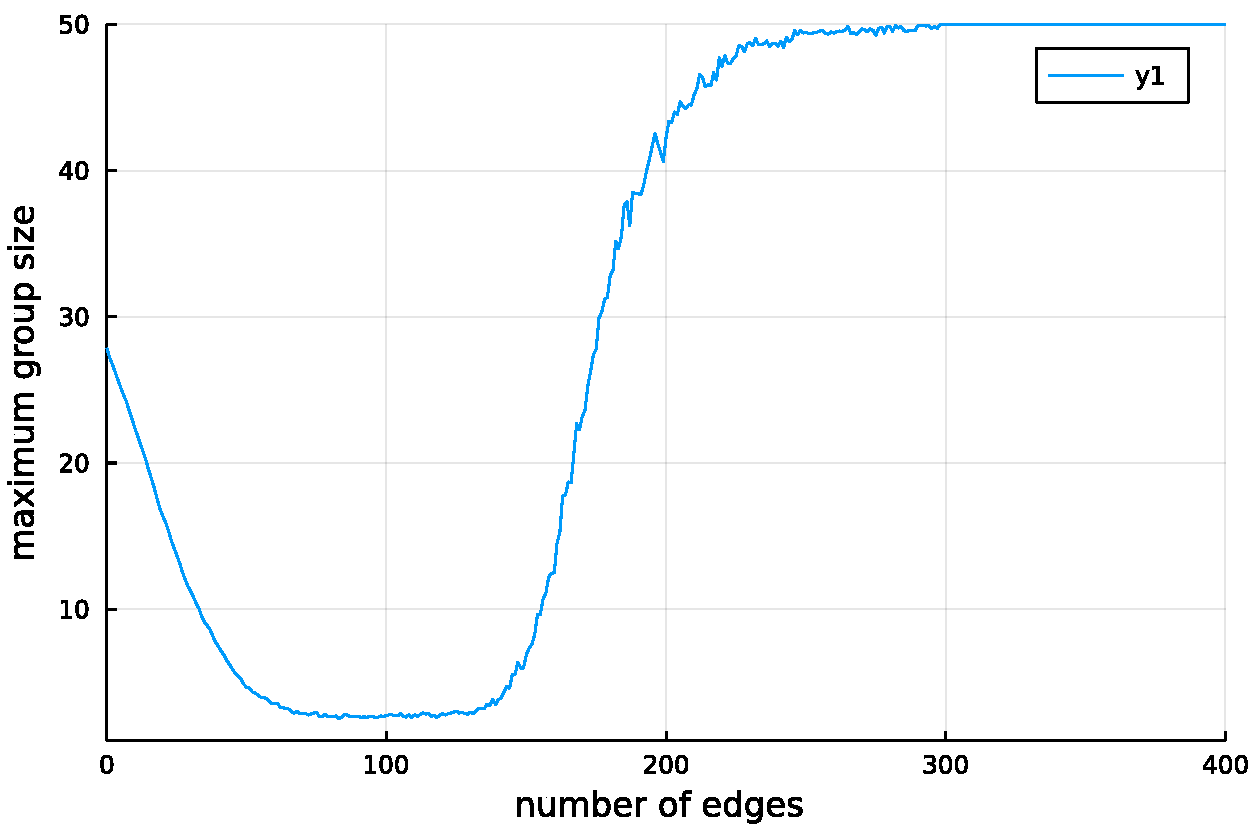
\includegraphics[keepaspectratio, scale=0.5]{images/edge-finite-maxsize-delta00003400.pdf}
      \subcaption{枝の本数と振動数によるクラスタの最大サイズの平均値の関係.}
      \label{fig:edge-cutting-K04-maxsize}
    \end{minipage}\\
    \begin{minipage}[b]{\linewidth}
      \centering
      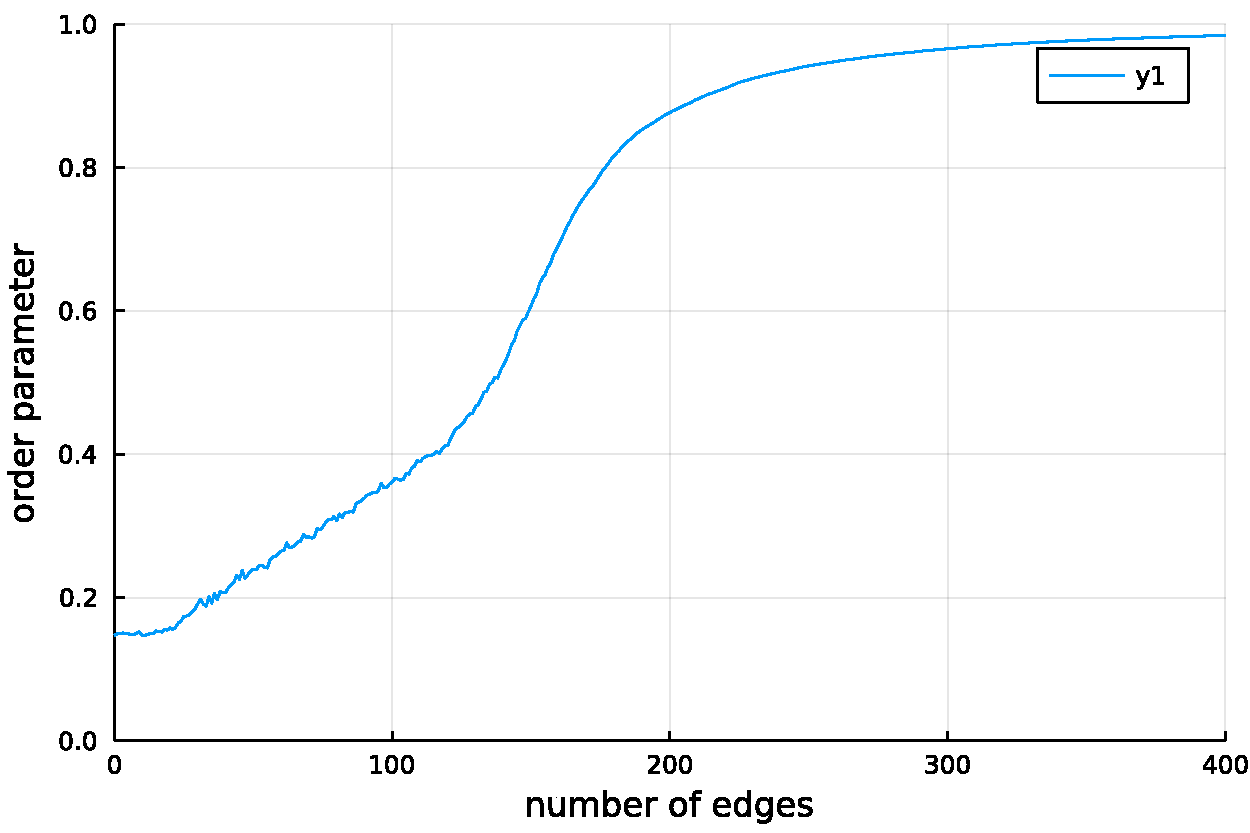
\includegraphics[keepaspectratio, scale=0.5]{images/edge-finite-R-delta00003400.pdf}
      \subcaption[c]{枝の本数とオーダーパラメータの平均値の関係.}
      \label{fig:edge-cutting-K04-R}
    \end{minipage}
    \caption{$n=50,\ \lambda=0.4,\ p=0.5$のときの枝の本数$m$と振動数によるクラスタの最大数とオーダーパラメータの$M=100$回平均値の関係を示す.
    ただし,実効振動数の差が$\Delta=0.00003$以内の振動子を同一クラスタとみなした.\\
    $0\leq m\leq 50$では,クラスタの最大サイズは線形に減少し,オーダーパラメータは緩やかに増加する.
    $50\leq m\lesssim 150$では,クラスタの最大サイズが極めて小さくなったまま変化せず,オーダーパラメータは$m=50$で変曲点を持ち$m<50$とは異なるペースで増加する.
    $150\lesssim m\lesssim 300$では,クラスタの最大サイズが急に増加し$n$に漸近する一方,オーダーパラメータは$m\sim 150$で変曲点を持ち,急激に増加し$1$に漸近する.
    }
    \label{fig:edge-cutting-K04}
\end{figure}

3つの同期状態に分かれている.それぞれの境界に相当する枝の臨界本数を$m_1,m_2$とすると以下のようにまとめられる.
$0\leq m<m_1$では最大集団のサイズ$L$が線形に減少し,オーダーパラメータ$R$は緩やかに増加する(Phase 1).
$m_1\leq m< m_2$では最大集団のサイズ$L$が極めて小さくなったまま変化せず,オーダーパラメータ$R$は Phase 1 とは異なるペースで増加する(Phase 2).
$m\geq m_2 $では最大集団のサイズ$L$は急激に増加し$n$に漸近し,オーダーパラメータ$R$も急激に増加し$1$に漸近する(Phase 3).
\section{同期状態の定性的解釈}
それぞれの同期状態は定性的に以下のように理解できる.
\renewcommand{\labelenumi}{Phase \theenumi}
\begin{enumerate}
    \item 固有振動数$\omega_\pm$の孤立した頂点が主な振動数となる.
    枝が1本増えるごとに高い確率で孤立した頂点をつなぐため,固有振動数$\omega_\pm$を実効振動数にもつ頂点数は平均$p$本減少する.
    よって,クラスタの最大サイズ$L$は
    \begin{equation}
        L(m)=np-mp     
    \end{equation}
    となる.
    一方,オーダーパラメータ$R$も枝の増加に伴う部分的同期により増加する.
    \item ネットワークがほとんど連結になるが,各試行で隣接した振動子の数及びその振動子の分布などのネットワーク構造が不均一であり異なる固有振動数を持つ振動子は同期しないため,ほとんどの振動子が異なるクラスタに属する.
    このため,クラスタの最大サイズ$L$は$L\approx 1$となり主要な振動数が存在しない.
    一方,オーダーパラメータ$R$は枝の増加に伴って実効振動数の分散が小さくなるため,増加する.
    \item 異なる固有振動数を持つ振動子同士が同期し始め,最後にはネットワーク全体が同期する.
    それに伴って,同期した振動子同士がクラスタを構成するため,クラスタの最大サイズ$L$は増加し,$n$に漸近する.
    オーダーパラメータ$R$も同期により実効振動数の分散が小さくなるため,増加する.
\end{enumerate}
\section{臨界本数}
\label{sec:percolate-m}
解析の都合上,$m_2,\ m_1$の順に調べる.
\subsection{最大サイズ$L$,オーダーパラメータ$R$が大きく変化する枝の本数$m_2$}
枝の本数$m$が頂点数$n$に比べ十分多い,特に,全ての振動子の次数が漸近的に等しいとき(\ref{sec:er-graph}節,Phase \ref{prev-er-phase4})を考える.
つまり,
\begin{equation}
    \label{eq:percolate-m2-assume}
    m= n\log n\ \omega(n)
\end{equation}
である.

このとき,振動子のネットワークを固有振動数$\omega_\pm$を持つ2種類の振動子が結合したものとして平均場近似することができる.
各振動子は確率$p$で$\omega_+$,確率$1-p$で$\omega_-$の固有振動数を持つとすると,それぞれの固有振動数を持つ振動子の数の平均はそれぞれ$np,\ n(1-p)$となる.
また,存在する枝のうち,異なる固有振動数の振動子同士をつなぐものは全体の$2p(1-p)$である.
以上より,固有振動数$\omega_+\ (\omega_-)$を持つ振動子の平均的な位相を$\phi_+\ (\phi_-)$とすると,平均場近似された2種類の結合振動子系のダイナミクスは以下のように表される.
\begin{align}
    \begin{split}
        \dot{\phi}_+&=\omega_++\frac{2p(1-p)m}{np}\lambda\sin(\phi_--\phi_+),\\
        \dot{\phi}_-&=\omega_-+\frac{2p(1-p)m}{n(1-p)}\lambda\sin(\phi_+-\phi_-).
    \end{split}
\end{align}
この同期条件は
\begin{equation*}
    \lambda\geq \frac{|\omega_+-\omega_-|n}{2m}
\end{equation*}
である,よって,
\begin{equation}
    \label{eq:percolate-m3}
    m_3=\frac{|\omega_+-\omega_-|n}{2\lambda}
\end{equation}
となる.
ただし,これは,$m_3$が式\eqref{eq:percolate-m2-assume}を満たすような結合強度のときのみ成立する.
つまり,
\begin{equation}
    \label{eq:er-meanfield-k}
    \lambda=(\omega_+-\omega_-)(\log n)^{-1}O(n^{-1})
\end{equation}
のときのような結合強度が十分弱い場合のみ成立する.
\subsection{最大サイズ$L$が下げ止まる枝の本数$m_1$}
\label{sec:percolate-m1}
クラスタの最大サイズ$L$は線形に減少する.
\begin{equation}
    L(m_1)=np-m_1p=0.
\end{equation}
よって,
\begin{equation}
    m_1=n
\end{equation}
となる.

しかしながら,$\lambda$が十分大きい場合は同期が開始し下げ止まるため,$m_1\leq n$となる.
特に$n\to\infty$の場合を考えると,$m=m_3$付近で
\begin{align}
    L(m)
    \begin{cases}
        \sim 1&(m<m_3),\\        
        =n'\gtrsim  1p&(m> m_3)        
    \end{cases}
\end{align}
となる,

振動子が$k$次である確率$P(k)\sim\binom{m}{k}(1/n)^k(1-1/n)^{m-k}$より,
$m< n$では,ほとんどの振動子の次数は$1$である.
よって,異なる固有振動数を持つ振動子と1つだけ結合した部分系が同期するか考えればよい.
同期条件は,
\begin{equation}
    \label{eq:percolate-2body}
    \lambda\geq\frac{|\omega_+-\omega_-|}{2}
\end{equation}
である.

ネットワークの一部の振動子が同期するとき,$m<n$であっても$L>np-mp$となる.
特に,式\eqref{eq:percolate-2body}が満たされるとき,連結になった振動子はほとんど同期するため,percolation が起こる$m=n/2$において$L>np-mp$となる.

以上より,ある$\lambda^1$が存在して,
\begin{align}
    m_1
    \begin{cases}
        \gtrapprox n/2&(\lambda \gtrsim |\omega_+-\omega_-|/2),\\        
        n'',\ (n/2<n''<n)&(|\omega_+-\omega_-|/2\gtrsim \lambda>\lambda^1),\\        
        n&(\lambda^1 \geq \lambda>1)        
    \end{cases}
\end{align}
となる.
\subsection{臨界本数の数値実験による確認}
$n=50,\ \lambda=0.4,\ p=1/2$について,$M=100$回試行し平均したものが図\ref{fig:edge-cutting-K04-maxsize}である.
$m_1=n=50$,$m_3\sim |\omega_+-\omega_-|n/2\lambda=250$となるが,概ね一致している.
$m_3$がクラスタの最大サイズ$L$が真に増加し始める$m$と一致しないのは,$n=50<\infty$という有限の振動子数を用いていること及び,$250< 50\log 50\ O(50)$であることに起因すると考えられる.

また,$n=50,\ \lambda=8,\ p=1/2$について,$M=100$試行し平均したものが図\ref{fig:edge-cutting-K8-maxsize}である.
図\ref{fig:edge-cutting-K8-maxsize}では,枝が繋がっていない孤立した振動子の数の平均値及び,連結な部分ネットワークのうち最大のものに属する振動子の数の平均値を重ねて表した.
ただし,枝が$m$本のときに連結な部分ネットワークのうち最大のものに属する確率$v$とすると,以下の式が成立することを用いた.
\begin{equation}
    v=1-\left( 1-\frac{2m}{n(n-1)}v \right)^{n-1}
\end{equation}
$\lambda$が$|\omega_+,\omega_-|/2$より十分大きい場合,異なる固有振動数を持つ振動子同士は結合すると必ず同期する.
そのため,枝の本数$m$が$0<m\lesssim n/2$では,枝の数が少ないため,孤立振動子が同じ実効振動数をもつクラスタの中で最大のサイズをもつクラスタとなる.
また,$m\gtrsim n/2$では連結な部分ネットワークは全て同期するため,連結な部分ネットワークのうち最大のものが,同じ実効振動数をもつクラスタの中で最大のサイズをもつクラスタとなる.
実際,理論的な2本の曲線と数値実験による曲線は概ね一致している.

\begin{figure}[tbp]
\centering
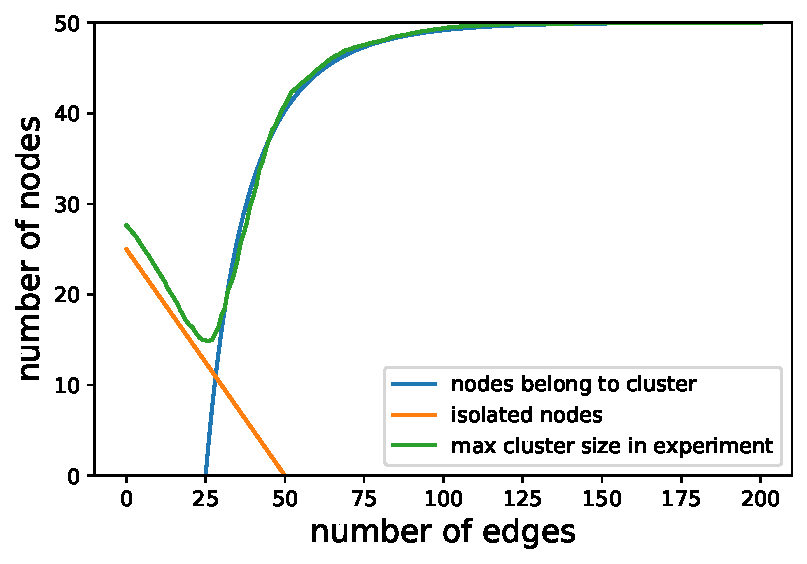
\includegraphics[width=105mm]{./images/edge-finite-maxsize-delta000038000-compare.pdf}
\centering
\caption{$n=50,\ \lambda=8,\ p=1/2$についてのクラスタの最大サイズの$M=100$試行平均値と枝の本数との関係を表した.
また,枝が繋がっていない孤立した振動子の数の平均値及び,連結な部分ネットワークのうち最大のものに属する振動子の数の平均値を重ねて表した.\\
$\lambda$が$|\omega_+,\omega_-|/2$より十分大きい場合,異なる固有振動数を持つ振動子同士は結合すると必ず同期する.
そのため,枝の本数$m$が$0<m\lesssim n/2$では,枝の数が少ないため,孤立振動子が同じ実効振動数をもつクラスタの中で最大のサイズをもつクラスタとなる.
また,$m\gtrsim n/2$では連結な部分ネットワークは全て同期するため,連結な部分ネットワークのうち最大のものが,同じ実効振動数をもつクラスタの中で最大のサイズをもつクラスタとなる.
実際,理論的な2本の曲線と数値実験による曲線は概ね一致している.}
\label{fig:edge-cutting-K8-maxsize}
\end{figure}

\section{議論}
\ref{sec:percolate-m}節で求めた臨界本数から以下のような定性的な理解ができる.
まず,最大クラスタが孤立振動子から構成される臨界本数$m_1$は,結合強度が十分弱い場合では孤立振動子がほとんどなくなるネットワークのサイズになる.
結合強度がある程度大きくなると,臨界本数は減少し,percolation が引き起こされるネットワークのサイズの半分の本数まで減少する.
そして,振動子が同期し始める境界である臨界本数$m_2$は,結合強度が十分弱い状況においては,結合強度が強く,固有振動数の差が小さいほど小さくなることがわかった.

このように,ネットワークにおけるクラスタサイズは,同期状態を調べるために用いられてきたオーダーパラメータよりも,顕著にネットワークにおけるミクロなダイナミクスを反映している.
したがって,ネットワークの構造の変化に伴う同期状態の変化を調べる上でクラスタサイズに注目することは有用であると考えられる.
\end{document}